\documentclass[letterpaper,10pt]{article}

\usepackage{titling}
\usepackage{listings}
\usepackage{url}
\usepackage{setspace}
\usepackage{subfig}
\usepackage{sectsty}
\usepackage{pdfpages}
\usepackage{colortbl}
\usepackage{multirow}
\usepackage{multicol}
\usepackage{relsize}
\usepackage{amsmath}
\usepackage{fancyvrb}
\usepackage{amsmath,amssymb,amsthm,graphicx,xspace}
\usepackage[titlenotnumbered,noend,noline]{algorithm2e}
\usepackage[compact]{titlesec}
\usepackage{XCharter}
\usepackage[T1]{fontenc}
\usepackage{tikz}
\usetikzlibrary{arrows,automata,shapes,trees,matrix,chains,scopes,positioning,calc}
\tikzstyle{block} = [rectangle, draw, fill=blue!20, 
    text width=2.5em, text centered, rounded corners, minimum height=2em]
\tikzstyle{bw} = [rectangle, draw, fill=blue!20, 
    text width=4em, text centered, rounded corners, minimum height=2em]

\newcommand{\CPP}{C\nolinebreak\hspace{-.05em}\raisebox{.4ex}{\tiny\bf +}\nolinebreak\hspace{-.10em}\raisebox{.4ex}{\tiny\bf +}}
\def\CPP{{C\nolinebreak[4]\hspace{-.05em}\raisebox{.4ex}{\tiny\bf ++}}}

\let\LaTeXtitle\title
\renewcommand{\title}[1]{\LaTeXtitle{\textsf{#1}}}


\addtolength{\oddsidemargin}{-1.000in}
\addtolength{\evensidemargin}{-0.500in}
\addtolength{\textwidth}{2.0in}
\addtolength{\topmargin}{-1.000in}
\addtolength{\textheight}{1.75in}
\addtolength{\parskip}{\baselineskip}
\setlength{\parindent}{0in}
\renewcommand{\baselinestretch}{1.5}

\singlespace

\begin{document}

\lecture{19 --- Query Optimization}{\term}{Jeff Zarnett}

\section*{Optimizing Database Queries}

Imagine you are given an assignment in a course and you are going to do it now. To get the assignment done, you will probably (1) figure out what exactly the assignment is asking you to do; (2) figure out how you are going to do it (e.g., must do part 1 first because part 2 depends on it...); and finally (3) do it! 

The goal of this topic is focused on step two of the process: figuring out how to do the assignment. We use the database and query optimization as an example, even though the topic is applicable in different contexts. This topic will not require you to have taken a databases course, though some familiarity with a SQL database will likely help with understanding. And depending on how the topic was covered in your database course\footnote{Or, you referred to my ECE 356 notes on Github to study for it...}, this might be entirely familiar. Okay, digression over. 

The procedure for the database server to carry out the query are the same~\cite{dsc}:

\begin{enumerate}
	\item Parsing and translation---interpreting the SQL query in a form the computer can work with.
	\item Optimization---figuring out how best to carry out the query.
	\item Evaluation---execution of the query according to the plan just developed.
\end{enumerate}

Usually a query is expressed in SQL, and that must then be translated into an equivalent internal expression using relational algebra. Relational algebra, super briefly, is just the set theory representation of database operations. Complex SQL queries are typically turned into \textit{query blocks}, which are translatable into relation algebra expressions. A query block has a single select-from-where expression, as well as related group-by and having clauses; nested queries are a separate query block~\cite{fds}.

A query like \texttt{SELECT salary FROM employee WHERE salary > 100000;} consists of one query block because it has only one part to it. We have possibilities. We can select all tuples where salary is more than 100~000 and then perform a projection of the salary field of that result (i.e., throw away the fields we do not need). The alternative is to do the projection of salary first and then perform the selection on the cut-down intermediate relation.

Suppose there is a subquery, like \texttt{SELECT name, street, city, province, postalCode FROM address WHERE id IN (SELECT addressID FROM employee WHERE department = 'Development');}. Then there are two query blocks, one for the subquery and one for the outer query. If there are multiple query blocks, then the server does not have to follow the same strategy for both.

What we need instead is a \textit{query execution plan}\footnote{\url{https://www.youtube.com/watch?v=fQk_832EAx4}, or \url{https://www.youtube.com/watch?v=l3FcbZXn4jM}}. To build that up, each step of the plan needs annotations that specify how to evaluate the operation, including information such as what algorithm or what index to use. An algebraic operation with the associated annotations about how to get it done is called an \textit{evaluation primitive}. The sequence of these primitives forms the plan, that is, how exactly to execute the query~\cite{dsc}. 

If there are multiple possible ways to carry out the plan, which there very often are, then the system will need to make some assessment about which plan is the best. It is not expected that users will write optimal queries; instead the database server should choose the best approach via \textit{query optimization}. Optimization is perhaps the wrong name for this because we are not choosing the \textit{optimal} approach; instead we will make some estimates about the query plans and try to choose the one that is most likely to be best. This suggests, as you may have guessed, we're going to use heuristics and consider trading accuracy for time.

\subsection*{Measures of Query Cost}

If you are asked to drive a car from point A to point B and there are multiple routes, you can evaluate your choices. To do so you need to break it down into different sections, such as drive along University Avenue, then get on Highway 85, then merge onto 401... Each segment has a length and a speed, such as knowing that you will drive 4 km along University Avenue and it is signed at 50 km/h (although with red lights and traffic and whatnot the actual average speed may be more like 30 km/h). By combining all of the segments, you get an estimate of how long that particular route will take. If you do this for all routes, you can see which route is the best. 

Of course, it may turn out that real life gets in the way: if there is a crash on the highway, traffic really sucks and your conclusion that taking this particular route would be fastest turns out to be wrong. Short of being able to see into the future, this is more or less inevitable: estimates are just informed opinions, and things may be worse (or better) than expected. 

Where does the time go in executing a query? The biggest component is most likely loading blocks from disk, considering how slow the disk operations are. Although we can improve this via use of SSDs, many large databases still use hard disk drives. CPU speeds are pretty fast, to the point even where memory accesses seem slow from the perspective of the CPU. So, no matter what we do, disk accesses likely account for far more of the time than CPU computation. In reality, CPU time is a nonzero part of query optimization, but we will ignore this (as does~\cite{dsc}) for simplicity's sake and use only the disk accesses to assess cost.

The number of block transfers (data moved in and out of memory) and the number of disk seeks (repositioning where on the disk we are reading from) are the important measures of interest here. SSDs have no seek time and have faster transfer speeds, but the number of block transfers is still relevant. To compute the estimate of how long we think it will take to perform an operation, the formula is $b \times t_{T} + S \times t_{s}$ where $b$ is the number of block transfers, $t_{T}$ is the time to transfer, $S$ is the number of seeks, and $t_{s}$ the time it takes to seek~\cite{dsc}. For a hard drive, transfer times are on the order of 0.1~ms and seek times are about 4~ms.

We will follow the estimating strategy in~\cite{dsc} which comes with a few caveats, explained in this paragraph. Sometimes writes can be twice as expensive as reads. This is because the disk subsystem may read back the written data to check that the write succeeded, but we will assume that does not happen here. Similarly, at this first level we are not including the amount of time it takes to write a final result back (that depends on the query... a select, for example, may not need it, where an update will). That cost would be accounted for separately. And the asterisk here is that the size of memory makes a big difference---if the buffer is large enough that all of the database fits in it, then disk reads are almost never needed. We will imagine the worst case scenario, that is, only one block per relation can be in memory at a time. If we are ``wrong'' and the data we need is already in memory, the actual cost is less than the estimated cost (which is better than the reverse). 

The estimates calculate only the amount of work that we think it will take to complete the operation. Unfortunately, there are several factors that will potentially affect the actual wall-clock time it takes to carry out the plan:

\begin{itemize}
	\item How busy the system is---if there are multiple concurrent operations then any particular operation may be queued or blocked or otherwise not able to proceed immediately, leading to a longer time to completion.
	\item What is in the buffer---if partial data is in the buffer that will speed up completion of the operation since some planned disk operations can be skipped.
	\item Data layout---if the data is packed well on disk then we need to do fewer seek operations (or shorter ones, perhaps); likewise, if the data is distributed over multiple physical disks we can sometimes do some reads in parallel, but it's hard to know exactly how much parallelization is possible.
\end{itemize}

You can probably think of various other factors that will affect the time it takes to execute the query in reality. The estimate is just an educated guess that we will use to plan how to do the work; it's not a promise of exactly how long it will take.

Note also that the lowest cost approach is not necessarily the fastest. Sometimes we can go faster by using more resources, but the approach the database often takes is the lowest cost (specifically, fewest disk reads). Recalling the earlier driving analogy, you can think of this as perhaps driving a longer route that involves more highway driving and therefore less time, even if it means more fuel consumption due to the increased distance and speed. When driving, we generally prefer to choose the lowest time estimate, but there are also people (``hypermilers'') who are really obsessed with getting maximum fuel economy... and the database is one of those people!

\subsection*{Alternative Routes}
There exist many different rules that allow transformation of a query into an equivalent. We're not focusing, here, on learning the rules as that would take us too far into the details about how the database actually works (or be redundant if you took a databases course that covered this already). But equivalency rules exist and resemble expression transformations that we learned in math class. Some of the equivalents are simple, multiplication commutes (e.g., $3 \times 10 \times 7$ is the same thing as $7 
\times 10 \times 3$) and others seemingly add extra complexity, but might be a useful way to approach the problem (e.g., $14 \times 13$ is equivalent to $14 \times 10 + 14 \times 3$). 

Suppose our query involves a selection and a join: we want to select the employee number, salary, and address for an employee with an ID of 385. Suppose number and salary are in the employee table with 300 entries, and the address information is in another table with 12000 entries. We have a join query, and if we do this badly, we will compute the join of employees and addresses, producing some 300 results, and then we need to do a selection and a projection on that intermediate relation. If done efficiently, we will do the selection and projection first, meaning the join needs to match exactly one tuple of employees rather than all 300. 

The query optimizer should systematically generate equivalent expressions, but since performing all possible transformations and then evaluating each option may itself take non-trivial time, it is likely that the optimizer does not consider every possibility and will take some ``shortcuts'' rather than brute force this. One technique that helps on top of that is to re-use common subexpressions to reduce the amount of space used by representing the expressions during evaluation~\cite{dsc}.

\subsection*{Estimating Statistics}

For all the discussion about how it might make sense to swap this or change that or do this rather than that, we have not yet really talked about how the system may guess about how many results are going to be returned. In the previous example I used exact numbers, 300... 1... 12000... etc., but for the database server to get those it can either look them up, or it can guess about them. As mentioned earlier, sometimes certain numbers, like the number of tuples in a relation, are easily available by looking at metadata. If we want to know, however, how many employees have a salary between \$40~000 and \$50~000, the only way to be sure\footnote{Other than nuking it from orbit...} is to actually do the query, and we most certainly do not want to do the query when estimating the cost, since at that point we might as well not bother optimizing at all.

If we cannot measure, then, well, we need to guess. Estimates are based on assumptions, and those assumptions are very often wrong. That is okay. We do not need to be perfect. All we need is to be better than not optimizing. And even if we pick the second or third or fifth best option, that is acceptable as long as we are close to the best option, more often than not.

There are five major areas where costs for actually performing a query accumulates. Some methods of estimation treat accessing disk storage as much larger than any other costs to the point where it's the only thing that is considered. That is not quite accurate, and modern query optimizers are capable of a more nuanced view. The list from~\cite{fds} below is more complete:

\begin{enumerate}
	\item \textbf{Disk I/O}: the previously-discussed costs of seeking and data transfer to get data from the disk or other secondary storage.
	\item \textbf{Disk Additional Storage}: the costs, if any, of storing intermediate relations on disk during processing of the query.
	\item \textbf{Computation}: The CPU usage that will be required to do the operations including sorting, merging, and arithmetic operations.
	\item \textbf{Memory}: The memory usage for the buffers necessary to do the desired operations.
	\item \textbf{Communication}: The cost of sending the results back to the requester, or in  a distributed database, the cost of transferring data between the different nodes.
\end{enumerate}

We will generally proceed on the basis that disk I/O is the largest cost and outweighs everything else. That may not be true in a particular use case (e.g., the database server has tons of RAM and a lot of data can be kept in memory). The principles of assessing cost and choosing a strategy still apply, even if we are optimizing faster queries or constrained by CPU instead of disk.

\paragraph{Metadata.} As previously mentioned, there is some metadata stored in the database that we could look at to find out some data that we know has some high accuracy. Some items that might be in the metadata, from~\cite{dsc} and ~\cite{fds}:

\begin{itemize}
	\item $n_{r}$: the number of tuples in a relation $r$ 
	\item $b_{r}$: The number of blocks containing a relation $r$ 
	\item $l_{r}$: the size in bytes of relation $r$
	\item $f_{r}$: the number of tuples of $r$ that fit into one block
	\item $V(A, r)$: the number of distinct values in $r$ of attribute $A$
	\item $h_{r, i}$: the height of an index $i$ defined on relation $r$
\end{itemize}

Some of these values can be computed, notably $l_{r}$ is the number of blocks times the size of a block, and $f_{r}$ is the number of tuples divided by the number of blocks. The value of $V(A, r)$ may or may not be maintained for all attributes, or for groups if that is so desired. If it is on a key field, every value is unique, so we know it is the same as the number of tuples for that field. There can also be metadata about index information as well... which might make it metametadata? 

There are obviously tradeoffs when it comes to maintaining metadata. The more often it is updated, the more effort is spent updating it. If every insertion or update or deletion resulted in an update, that may mean a nontrivial amount of time is spent updating this data. If we only do periodic updates, it likely means that the statistic data will be outdated when we go to retrieve it for use in a query optimization context. Perhaps some amount of balance is necessary: updates can be done during times of lower system load with some maximum limit for how long an update can wait before it gets enough priority. This is, in some small way, a callback to scheduling algorithms you have surely learned about in an OS class. 

A database may also be interested in keeping some statistical information in a histogram. The values are divided into ranges and we have some idea of how many tuples are in those ranges. You have almost certainly seen a histogram before in something like a population pyramid diagram. An example from~\cite{dsc}:

\begin{center}
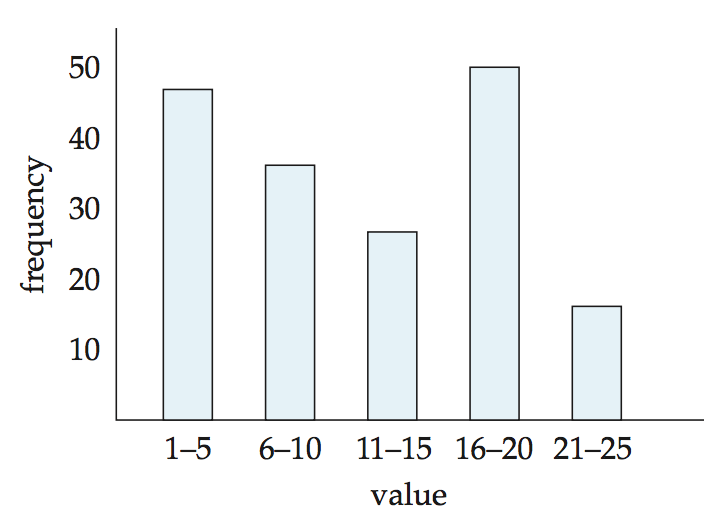
\includegraphics[width=0.4\textwidth]{images/histogram}
\end{center}

That should also tell you that they do not necessarily have an even distribution. A histogram does not take up a lot of space and it can help us to figure out certain problems: if we have a histogram of salaries and the largest bucket is 100~000+ and there are 10 people in this category, and there is a query asking how many employees have a salary greater than or equal to \$100~000 we will know at least that the number of tuples to be returned is 10. Nice.

The above numbers are exact values which we can know and, hopefully, trust although they could be slightly out of date depending on when exactly metadata updates are performed. The more exact values we have, the better our guesses. But things start to get interesting when, in the previous example, we ask something that does not have a category, such as how many people have a salary larger than \$150~000, where there isn't an obvious answer found in the metadata?

\subsection*{Join Elimination}

You may ask, of course, why should the optimizer do this work at all? Why not simply count on the developers who wrote the SQL in the first place to refactor/change it so that it is no longer so inefficient? That would be nice but would you also like a pony?  Developers make mistakes, as you know, or perhaps some legacy code cannot be changed for some reason. Regardless, SQL is a language in which you specify the result that you want, not specifically how to get it. If there is a more efficient route, then it's worth taking from the point of view of the database server. The same logic applies in the compiler, incidentally; if you ask for some operation that the compiler knows it can replace with an equivalent but faster operation, why wouldn't you want that? Compilers don't admonish the user for writing code that it has to transform into a faster equivalent, they just do that transparently. You're welcome!

Our guide in this is~\cite{joinelim}. We will examine some real SQL queries to see how we can get rid of a total unnecessary join. This join can only be removed if the database server can prove that the join is not needed and that therefore the removal of this operation has no impact on the outcome.


Consider a statement that looks like this: \texttt{SELECT c.* FROM customer AS c JOIN address AS a ON c.address\_id = a.address\_id;} This gets customer information and joins with those where there are addresses on file. This is an inner join and as presented, we cannot do any elimination with this information. We need to make sure that the customer data has a matching row.

If, however, a new piece of information is considered, it changes everything entirely. Suppose that we have a foreign key defined from customer's \texttt{address\_id} to the address \texttt{id} field. If nulls are not permitted then we know for sure that every customer has exactly one record in the address table and therefore the join condition is not useful and may be eliminated. This means we could in fact replace that query with \texttt{select * from customer;} with no need for any references to the join table at all. That would be much, much faster since it is a simple select with no conditions.

The foreign key and not null constraints on the address ID field of the customer make it possible for the optimization of the join elimination to occur.

An outer join constraint can be removed as well. Imagine the query said this: \texttt{SELECT c.* FROM customer AS c LEFT OUTER JOIN address AS a ON c.address\_id = a.address\_id;}. All tuples are fetched from customer whether or not there is an associated address. Once again, if the foreign key constraint and not-null properties hold for this field it means that we can perform the equivalent transformation and replace the join query with a simple unqualified select. 

Suppose the foreign key constraint is removed. Does that change anything? No---a unique constraint on the address would be sufficient for us to conclude that the join means no duplication of rows in customer will take place. Therefore it can once again be replaced with the simple \texttt{select * from customer;}.

If, however, both constraints are removed and we cannot be sure that there is at most one address corresponding to a customer, then we have no choice but to do the join.

Obviously, the more complex the query, the harder it is to determine whether or not a particular join may be eliminated. More than that, the same queries written exactly the same on a database in which the constraints have not been added would not be eligible for the join elimination optimization. In the inner join example, the foreign key and not null constraints, for example, are beneficial. This reveals a second purpose why constraints are valuable in the database. In addition to allowing us to enforce logical rules of the application inside of the database, it allows queries to be completed more efficiently.

Perhaps an analogy helps. You are asked to search through the library to find all copies of the book ``Harry Potter and the pthread House Elves''. That is a plausible task. But, suppose that you know as well there is a rule that this library will keep only one copy of that book ever. If that is the case, as soon as you have found the single copy of that book, you can stop looking (no need to check more ``just in case''). This sort of optimization is very similar in that the rules let us avoid doing unnecessary work and that is a big part of the optimization routine.

\subsection*{Evaluation Plan Selection}

It was perhaps oversimplifying to have said earlier that choosing a plan was just as simple as picking the one with the lowest cost. There is a little bit more to it than that. The point about choosing the one with the lowest cost is correct (generally), but the difficulty is in devising and calculating all possible evaluation plans. Neither devising nor analyzing alternatives is free in terms of CPU usage or time, and it is possible to waste more time on analysis than a better plan would save. 

A simplified approach, then, focuses just on what order in which join operations are done and then how those joins are carried out. The theory is that the join operations are likely to be the slowest and take the longest, so any optimization here is going to have the most potential benefit.

We already know that the order of joins in a statement like $r_{1} \bowtie r_{2} \bowtie r_{3}$ is something the optimizer can choose. In this case there are 3 relations and there are 12 different join orderings. In fact, for $n$ relations there are $\dfrac{(2(n-1))!}{(n-1)!}$ possible orderings~\cite{dsc}. Some of them, are symmetric, which reduces the number that we have to calculate, since $r_{1} \bowtie r_{2}$ is not different from $r_{2} \bowtie r_{1}$ (in relational algebra). In any case, even if we can cut down the symmetrical cases the problem grows out of hand very quickly when $n$ gets larger. 

Once more than three relations are affected by a join query it may be an opportunity to stop and think very hard about what is going on here, because this is quite unusual if the database design is good. The database server may want to ask why do you have a join query that goes across six or eight or twelve relations, but the database server (sadly) does not get to write the developers a nasty resignation letter saying that it can't continue to work this hard due to the negative effects on its health. It will dutifully do the work you asked it to and even try to make the best of this inefficient situation by optimizing it. But clearly it cannot examine all (non-symmetric) approaches and choose the optimal one. It would take too long.

Fortunately, we can create an algorithm that can ``remember'' subsets of the choices. If we have, for example, $r_{1} \bowtie r_{2} \bowtie r_{3} \bowtie r_{4} \bowtie r_{5}$ and the database server does not segmentation fault in disgust, we can break that down a bit. We could compute the best order for a subpart, say $(r_{1} \bowtie r_{2} \bowtie r_{3})$ and then re-use that repeatedly for any further joins with $r_{4}$ and $r_{5}$~\cite{dsc}. This ``saved'' result can be re-used repeatedly turning our problem from five relations into two three-relation problems.

This is a really big improvement, actually, considering how quickly the factorial term scales up. The trade-off for this approach is that the resultant approach may not be globally optimal (but instead just locally optimal). If $r_{1} \bowtie r_{4}$ produces very few tuples, it may be maximally efficient to do that join computation first, a strategy that will never be tried in an algorithm where $r_{1}$, $r_{2}$, and $r_{3}$ are combined to a subexpression for evaluation. 

Remember though, this is as estimating process. The previous statement that said $r_{1} \bowtie r_{4}$ produces very few tuples as if it is a fact. The optimizer does not know that for sure and must rely on estimates where available. So even though the optimizer may, if it had tried all possibilities, determined that $r_{1} \bowtie r_{4}$ produces the fewest tuples and should be joined first, it is possible that estimate was off and the actual cost of a different plan was lower.

The sort order in which tuples are generated is important if the result will be used in another join. A sort order is called \textit{interesting} if it is useful in a later operation. If $r_{1}$ and $r_{2}$ are being computed for a join with $r_{3}$ it is advantageous if the combined result $r_{1} \bowtie r_{2}$ is sorted on attributes that match to $r_{3}$ to make that join more efficient; if it is sorted by some attribute not in $r_{3}$ that means an additional sort will be necessary~\cite{dsc}.

With this in mind it means that the best plan for computing a particular subset of the join query is not necessarily the best plan overall, because that extra sort may cost more than was saved by doing the join itself faster. This increases the complexity, obviously, of deciding what is optimal. Fortunately there are, usually anyway, not too many interesting sort orders~\cite{dsc}. 

\subsubsection*{Generating Alternatives}

Join order optimization is a big piece of the puzzle but it's not the only thing we can do in query evaluation. Let's briefly revisit the subject of how equivalent queries are formed. We already decided it is too expensive to try out all equivalent queries, but perhaps we are determined to try to at least generate lots of alternatives. The textbook~\cite{dsc} summarizes some strategies from the Volcano research project that would make it possible to generate a larger number of plans than we might otherwise be able to. We need four things.

\begin{enumerate}
	\item A way of storing expressions that reduces duplication and therefore keeps down the amount of space needed to store the various queries.
	\item A way of detecting duplicate derivations of the same expression.
	\item A way of storing optimal subexpression evaluation plans so that we don't have to recompute them.
	\item An algorithm that will terminate the evaluation of a particular plan early if it is already worse than the cheapest plan found so far.
\end{enumerate}

The details are obviously a bit complex. Most of this is beyond what we will discuss in this course, but some of those things we have already seen. For example, the algorithm earlier has got a way of storing evaluations of sub expressions so that we can re-use them. It could be modified to terminate earlier if, for example, the individual costs of \texttt{r1} or \texttt{r2} were already larger than the known stored plan.

\subsubsection*{Nested Subqueries}

On the subject of generating alternatives, if possible, nested subqueries will be transformed into an alternative representation: a join query. To summarize the rather long story, if evaluated the ``slow'' way the subquery needs to be run a lot of times. Thus, to make it faster, we would prefer to turn it into a join (which we already know how to handle). If really necessary we can run the subquery once and use that temporary relation in a join (where exists or ``in'' predicates may fall into this category).

Suffice it to say that transformation of nested queries is complicated and it may mean that the optimizer is unable to find some efficient route for executing the desired query if the query is complex. If possible, nested queries should be avoided. Sometimes you don't have much choice however. Amusingly, many years ago, MySQL did not support subqueries and that was one way to force people to come to grips with how to use joins. But somehow I do not think MySQL was intentionally doing anyone a favour, any more than having a terrible optimizer ``forces'' developers to write better queries. 


\subsubsection*{Shortcuts}

Now we will talk about some heuristic rules (guidelines, really) that we have definitely mentioned earlier when we talked about, for example, how to perform a selection. Now we can actually discuss them more formally.

\paragraph{Perform selection early.} No surprises here: the sooner we do a selection, the fewer tuples are going to result and the fewer tuples are input to any subsequent operations. Performing the selection is almost always an improvement. Chances are we get a lot of benefit out of selection: it can cut a relation down from a very large number of tuples to relatively few (or even one). 

There are exceptions, however. One from~\cite{dsc}: suppose the query is $\sigma_{\theta}( r \bowtie s )$ where $\theta$ refers only to attributes in $s$. If we do the selection first and (1) $r$ is small compared to $s$ and (2) there is an index on the join attributes of $s$ but not on those used by $\theta$ then the selection is not so nice. It would throw away some useful information and force a scan on $s$; it may be better to do the join using the index and then remove tuples with the selection.

\paragraph{Perform projection early.} Analogous to the idea of doing selection early, performing projection early is good because it tosses away information we do not need and means less input to the next operations. Just like selection, however, it is possible the projection throws away an attribute that will be useful. If the query does not ask for the join attribute in the output (e.g., does it matter what a person's address ID is?) then that join attribute will need to be removed from the output but if removed too soon it makes it impossible to do the join.

\paragraph{Set limits.} Another strategy for making sure we choose something appropriate within a reasonable amount of time is to set a time limit. Optimization has a certain cost and once this cost is exceeded, the process of trying to find something better stops. But how much time to we decide to allocate? A suggested strategy from~\cite{dsc} says to use some heuristic rules to very quickly guess at how long it will be. If it will be very quick then don't bother doing any further searching, just do it. If it will be moderate in cost, then a moderate optimization budget should be allocated. If it is expensive then a larger optimization budget is warranted.

\paragraph{Plan caching.} In any busy system, common queries may be repeated over and over again with slightly different parameters. For example, \cite{dsc} suggests the following sort of query: a student wishes to query what courses they are enrolled in. If one student does this query with a particular value for student ID number, we can re-use that same evaluation plan in the future when another student does the exact same query with her student ID number instead. 

The results will be different and this query may be more expensive on the second run if, for example, the second student is taking 7 courses this term and the first student is taking 5. That is expected, all we really needed was an estimate. With that in mind, if we have actually carried out the exact query we can use the actual execution time as the updated estimate for how long it takes (or perhaps an average of the last $n$ executions of that same query if it has high variability). 

\subsection*{Applicability}
If we're not planning on implementing or understanding a database, is any of this useful? Yes! The database is just a specific example of an implementation and something that we're familiar with. The real lesson is about how to programmatically generate, evaluate, and choose amongst alternative options for accomplishing a goal. 

\bibliographystyle{alphaurl}
\bibliography{459}


\end{document}
